\section{Results and discussion}
The development of the bird classifier using cased-based reasoning has
been successful in many ways. The final version met all the initial requirements
stated at the beginning of the project and the code has a low footprint while
providing an adequate performance.



\begin{figure}[htp]
    \subfloat[Canberra. \fontfamily{qcr}\selectfont \newline 1.0 * FFT Peak 1]{
      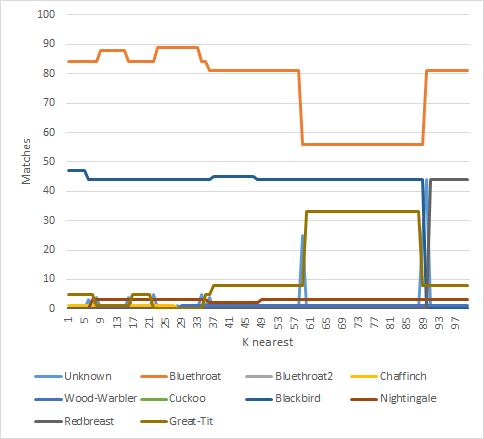
\includegraphics[clip,width=0.4\columnwidth]{eval-canberra-0_0-0_0-1_0-0_0-0_0-0_0-0_0-0_0}
    }
    ~
    \subfloat[Canberra. \fontfamily{qcr}\selectfont \newline 1.0 * FFT Peak 1 \newline 1.0 * FFT Peak 1 Delta]{
      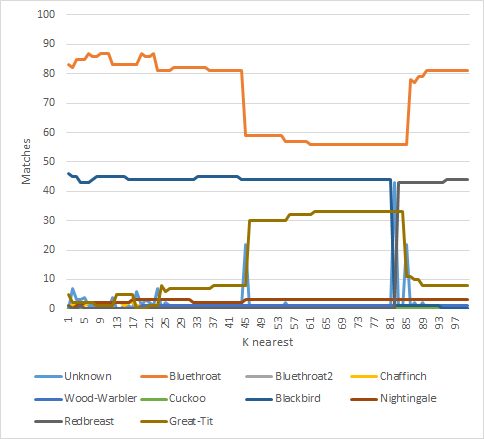
\includegraphics[clip,width=0.4\columnwidth]{eval-canberra-0_0-0_0-1_0-0_0-1_0-0_0-0_0-0_0}
    }
    \caption{Results. Comparing 127 samples of Bluethroat2 to the case database. Y-axis is the number matches for each bird class.
    This shows adding FFT Peak 1 Delta does not yield that better result.}
    \label{fig:results}
\end{figure}

\begin{figure}[htp]

  \subfloat[Canberra. \fontfamily{qcr}\selectfont \newline 0.1 * FFT Area Delta. \newline 1.0 * FFT Peak 1 Delta]{
    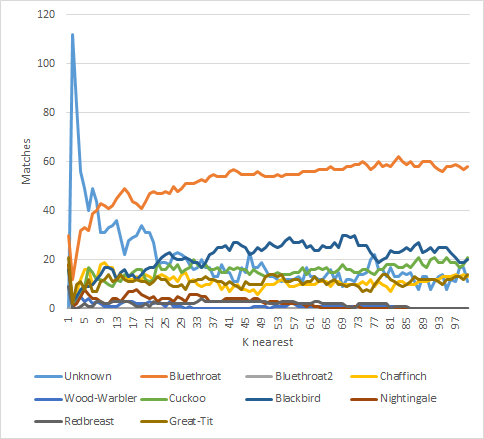
\includegraphics[clip,width=0.4\columnwidth]{eval-canberra-0_0-0_1-0_0-0_0-1_0-0_0-0_0-0_0}
  }
  ~
  \subfloat[Canberra. \fontfamily{qcr}\selectfont \newline 1.0 * FFT Area Delta. \newline 1.0 * FFT Peak 1 Delta]{
    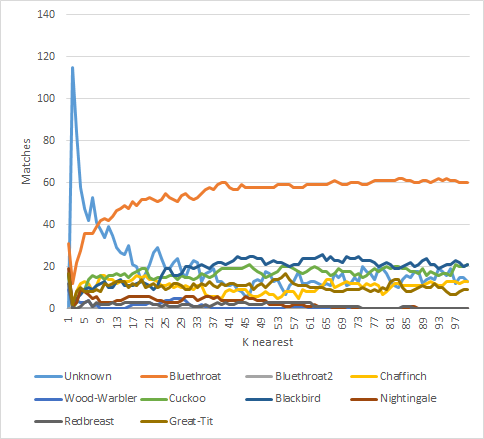
\includegraphics[clip,width=0.4\columnwidth]{eval-canberra-0_0-1_0-0_0-0_0-1_0-0_0-0_0-0_0}
  }
    \caption{Results. This shows a good combinations of weight. Note that FFT Peak 1 Delta is very neccery.}
    \label{fig:results}
\end{figure}



\begin{figure}[htp]
    \subfloat[Canberra. \fontfamily{qcr}\selectfont \newline 1.0 * FFT Peak 1 Delta]{
      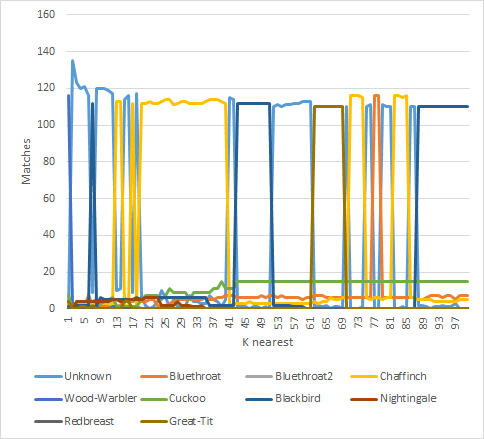
\includegraphics[clip,width=0.4\columnwidth]{eval-canberra-0_0-0_0-0_0-0_0-1_0-0_0-0_0-0_0}
    }
    \caption{Results. Note that FFT Peak 1 Delta alone does not yield acceptable result.}
    \label{fig:results}
\end{figure}




\begin{figure}[htp]
    \subfloat[Canberra. \fontfamily{qcr}\selectfont \newline 1.0 * FFT Area Delta \newline 0.1 * FFT Peak 1]{
      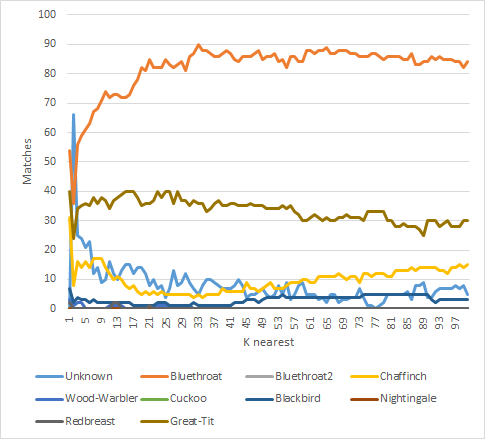
\includegraphics[clip,width=0.4\columnwidth]{eval-canberra-0_0-1_0-0_1-0_1-1_0-0_0-0_0-0_0}
    }
    ~
    \subfloat[Canberra. \fontfamily{qcr}\selectfont \newline 1.0 * FFT Area Delta \newline 1.0 * FFT Peak 1]{
      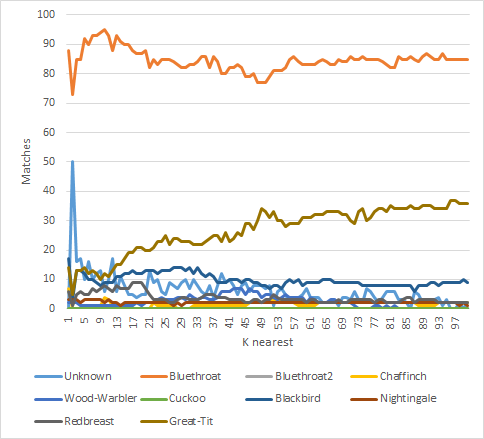
\includegraphics[clip,width=0.4\columnwidth]{eval-canberra-0_0-1_0-1_0-0_0-0_0-0_0-0_0-0_0}
    }

    \subfloat[Canberra. \fontfamily{qcr}\selectfont \newline 1.0 * FFT Area Delta \newline 1.0 * FFT Peak 1  \newline 1.0 * Peak 1 Delta]{
      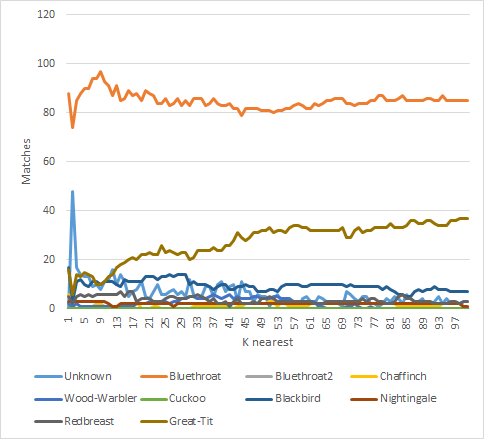
\includegraphics[clip,width=0.4\columnwidth]{eval-canberra-0_0-1_0-1_0-0_0-1_0-0_0-0_0-0_0}
    }
    \caption{Results.}
    \label{fig:results}
\end{figure}


\begin{figure}[htp]
    \subfloat[Canberra. \fontfamily{qcr}\selectfont \newline 1.0 * FFT Area \newline 1.0 * FFT Area Delta \newline 1.0 * Peak 1 \newline 1.0 * Peak 2 \newline 1.0 * Peak 1 Delta]{
       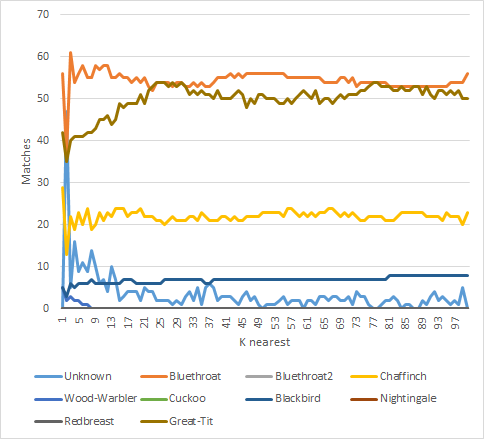
\includegraphics[clip,width=0.4\columnwidth]{eval-canberra-1_0-1_0-1_0-1_0-1_0-0_0-0_0-0_0}
    }
    ~
    \subfloat[Euclidean. \fontfamily{qcr}\selectfont \newline 1.0 * FFT Area \newline 1.0 * FFT Area Delta \newline 1.0 * Peak 1 \newline 1.0 * Peak 2 \newline 1.0 * Peak 1 Delta]{
      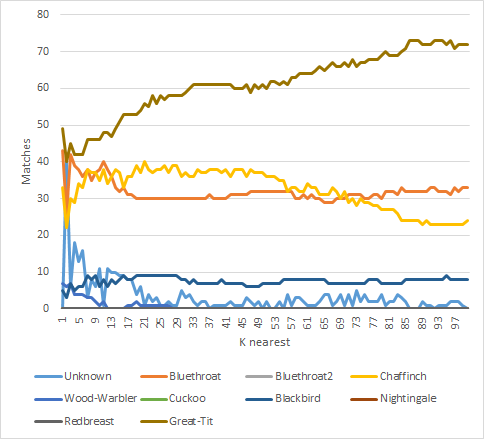
\includegraphics[clip,width=0.4\columnwidth]{eval-euclidean-1_0-1_0-1_0-1_0-1_0-0_0-0_0-0_0}
    }

    \subfloat[Euclidean. \fontfamily{qcr}\selectfont \newline 1.0 * FFT Area \newline 1.0 * FFT Area Delta \newline 1.0 * Peak 1 \newline 1.0 * Peak 2 \newline 1.0 * Peak 1 Delta \newline 1.0 * Mean \newline 1.0 * STD]{
      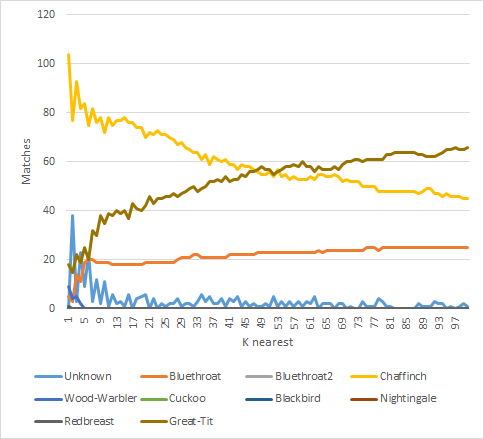
\includegraphics[clip,width=0.4\columnwidth]{eval-euclidean-1_0-1_0-1_0-1_0-1_0-1_0-1_0-0_0}
    }
    \caption{Results.}
    \label{fig:results}
\end{figure}

\begin{figure}[htp]
    \subfloat[Euclidean. \fontfamily{qcr}\selectfont \newline 1.0 * FFT Area \newline 1.0 * FFT Area Delta \newline 1.0 * Peak 1 \newline 1.0 * Peak 2 \newline 1.0 * Peak 1 Delta \newline 1.0 * Mean \newline 1.0 * STD \newline 1.0 * ZCR]{
      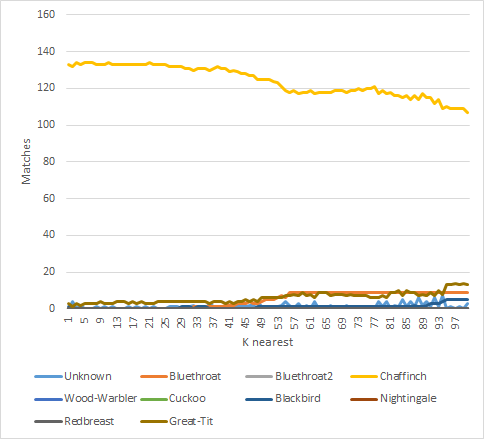
\includegraphics[clip,width=0.4\columnwidth]{eval-euclidean-1_0-1_0-1_0-1_0-1_0-1_0-1_0-1_0}
    }
    ~
    \subfloat[Canberra. \fontfamily{qcr}\selectfont \newline 1.0 * FFT Area \newline 1.0 * FFT Area Delta \newline 1.0 * Peak 1 \newline 1.0 * Peak 2 \newline 1.0 * Peak 1 Delta \newline 1.0 * Mean \newline 1.0 * STD \newline 1.0 * ZCR]{
      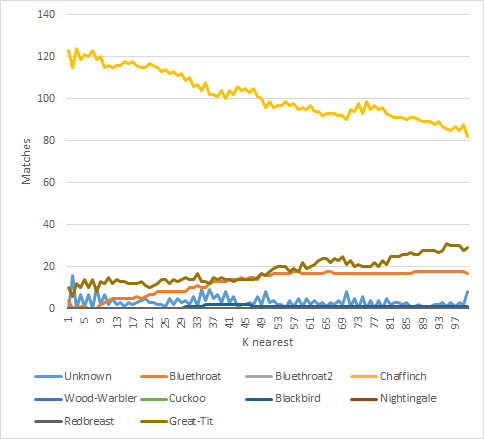
\includegraphics[clip,width=0.4\columnwidth]{eval-canberra-1_0-1_0-1_0-1_0-1_0-1_0-1_0-1_0}
    }

    \subfloat[Manhattan. \fontfamily{qcr}\selectfont \newline 1.0 * FFT Area \newline 1.0 * FFT Area Delta \newline 1.0 * Peak 1 \newline 1.0 * Peak 2 \newline 1.0 * Peak 1 Delta]{
      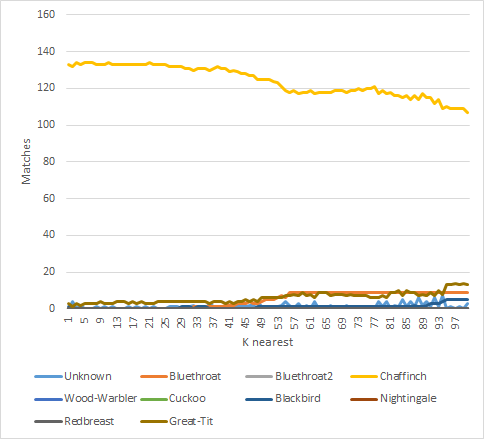
\includegraphics[clip,width=0.4\columnwidth]{eval-manhattan-1_0-1_0-1_0-1_0-1_0-0_0-0_0-0_0}
    }
    \caption{Results.}
    \label{fig:results}
\end{figure}

The test has showed that it is possable to classify a noisy, different audio strength Bofink compared to a database with no noize and high quality audio sounded birds.

The tests shows that using euclidian and manhattan distance does not yield accurate results.
Multiple test with canberra distance with different weight configuration have the most accurate result.

List of possable high accuracy configuration.
These configurations is found by trial and error and therefore should not be the perfect result.
Config 1: Canberra, 1.0 * FFT Peak 1 Delta, 1.0 * FFT Area Delta.
Config 2: Canberra, 1.0 * FFT Peak 1.
Config 3: Canberra, 1.0 * FFT Peak 1, 1.0 * FFT Area Delta.
Config 4: Canberra, 1.0 * FFT Area Delta, 0.2 * FFT Peak 1, 0.1 * FFT Peak 2, 1.0 * FFT Peak 1 Delta

\section{Discussion}
Config 4 is currently the best mean accuracy over K from 1 to 100.
Some feature can not act alone. FFT Peak 1 can get high accurcy alone. When FFT Peak 1 is combined with other features the result can get better if the weight is lowered for FFT Peak 1. This conclude that that a dominating feature like FFT Peak 1 may not seem that important. It is important not to get biased for a feature even if that feature alone gives better result than the others.
